\documentclass[linenumbers, twocolumn]{aastex631}

\usepackage{graphicx}
\usepackage{amsmath}
\usepackage{amssymb}
\usepackage{newtxtext,newtxmath}
\usepackage{hyperref}
\usepackage{gensymb}
\usepackage{enumitem}

\newcommand{\vdag}{(v)^\dagger}
\newcommand\aastex{AAS\TeX}
\newcommand\latex{La\TeX}

\newcommand{\Msun}{\ensuremath{M_{\odot}}}
\newcommand{\Gyr}{\ensuremath{\textrm{Gyr}}}
\newcommand{\Myr}{\ensuremath{\textrm{Myr}}}
\newcommand{\yr}{\ensuremath{\textrm{yr}}}
\newcommand{\kpc}{\ensuremath{\textrm{kpc}}}
\newcommand{\pc}{\ensuremath{\textrm{pc}}}
\newcommand{\kms}{\ensuremath{\textrm{km}/\textrm{s}}}
\newcommand{\tocite}{\textcolor{blue}{cite}}
\newcommand{\FeH}{\ensuremath{[\textrm{Fe}/\textrm{H}]}}
\newcommand{\MgFe}{\ensuremath{[\textrm{Mg}/\textrm{Fe}]}}
\newcommand{\OFe}{\ensuremath{[\textrm{O}/\textrm{Fe}]}}
\newcommand{\alphaFe}{\ensuremath{[\alpha/\textrm{Fe}]}}
\newcommand{\tform}{\ensuremath{t_{\textrm{form}}}}
\newcommand{\dex}{\ensuremath{\textrm{dex}}}
\newcommand{\Msunyr}{\ensuremath{\Msun/\textrm{yr}}}

\newcommand{\red}[1]{\textcolor{red}{#1}}

% \received{March 1, 2021}
% \revised{April 1, 2021}
%\accepted{\today}

\shorttitle{The Milky Way's Phoenix Phase}
\shortauthors{Beane et al.}

\graphicspath{{./}{fig/}}

\begin{document}

\title{Something something}

\author{Angus Beane}
\affiliation{Center for Astrophysics $|$ Harvard \& Smithsonian, Cambridge, MA, USA}

\author{James W. Johnson}
\affiliation{The Observatories of the Carnegie Institution for Science, Pasadena, CA, USA}

\author{Vadim Semenov}
\affiliation{Center for Astrophysics $|$ Harvard \& Smithsonian, Cambridge, MA, USA}

\author{Lars Hernquist}
\affiliation{Center for Astrophysics $|$ Harvard \& Smithsonian, Cambridge, MA, USA}

\author{et al}

\begin{abstract}
    The Milky Way is known to host at least two modes in the present day distribution of chemical abundances. The exact cause of this bimodality is disputed, but one class of explanations involves the merger between the Milky Way and a relatively massive sattelite (Gaia-Sausage-Enceladus) at $z\sim2$. However, reproducing this bimodality in simulations is not straightforward, with conflicting results on the prevalance, morphology, and mechanism behind multimodality. We present a case study of a galaxy at $z=1.5$ in the Illustris TNG50 simulation which undergoes a starburst and brief quiescent phase. In the fiducial simulation, this galaxy does not host any multimodality in its chemical abundance plane. However, when an artificial slope in \alphaFe{} as a function of time is added (older stars are given boosted \alphaFe{}), we show that the distribution becomes strikingly multimodal. This suggests that, for this creation avenue, multimodality can only be created at times when \alphaFe{} is rapidly declining, as expected at high-$z$. It also provides additional support that models must produce galaxies with this declination. We suggest that TNG50 fails in this respect because the resolved star formation efficiency at high densities is too low.
  \end{abstract}
    
  \keywords{Classical Novae (251) --- Ultraviolet astronomy(1736) --- History of astronomy(1868) --- Interdisciplinary astronomy(804)}
  

\section{Introduction}\label{sec:intro}
For most elements, their stellar surface abundances retain the composition of their natal gas cloud. Therefore, the present-day distribution of stellar surface abundances encodes the chemical history of a galaxy. Two elements have received particular interest in the Milky Way: Fe and $\alpha$-elements (elements produced through the $\alpha$-process). Fe is produced in both Type Ia and Type II SNe whereas $\alpha$-elements are produced predominantly through Type II SNe. Because these SNe occur on different timescales (10s of Myr after star formation for Type II, as compared to 100s of Myr for Type Ia), the ratio between $\alpha$-elements and Fe generally decreases with time.

This decline of \alphaFe{} over time has long been recognized \citep{1979ApJ...229.1046T}. This trend is only generally true, though, with non-monotonic behavior observed in observations and even one-zone chemical models \citep[e.g.][]{2022arXiv220402989C}. 

Two types of supernovae (SNe) are responsible for most of the production of Fe and $\alpha$-elements: Type II and Type Ia \citep{2023A&ARv..31....1A}. Type II SNe originate from massive stars whose lifetimes are rather short (10s of Myr). Type Ia SNe, on the other hand, are thought to originate from white dwarfs whose masses have exceeded the Chandrasekar limit due to accretion from a donor star.

\section{Methods}\label{sec:methods}
\subsection{IllustrisTNG Sample}\label{ssec:tng}
We have made use of the Illustris TNG50 simulation \citep{2019MNRAS.490.3196P, 2019MNRAS.490.3234N}, a cosmological simulation of a $\sim50\,\textrm{cMpc}$ box at high resolution ($m_{\textrm{baryon}}\sim8.5\times10^4\,\Msun$) It uses the gravito-magneto-hydrodynamics code \texttt{AREPO} \citep{2010MNRAS.401..791S, 2016MNRAS.455.1134P}, along with the TNG model \citep{2017MNRAS.465.3291W, 2018MNRAS.473.4077P}. This model includes several subgrid processes: a wind generation model, chemical enrichment from supernovae and asymptotic giant branch stars, and thermal and kinetic feedback from AGN.

Using the public catalog, we selected a sample of subhalos at $z=1.5$ (snapshot 40) according to the following criteria: (1) the subhalo is central (i.e., the most massive subhalo within its halo), and (2) the subhalo's stellar mass is between $10^{10}$ and $10^{10.5}\,\Msun/\textrm{h}$. There were a total of 168 subhalos that met both criteria. The chosen mass range is broadly consistent with the expected mass of the Milky Way at this redshift \citep{2013ApJ...771L..35V}. We chose to make our selection of galaxies at $z=1.5$ instead of at lower redshift because we wished to capture the \textit{formation} of any multimodal structure. We did not want contamination by mergers at lower redshift which we know contribute very little to the Milky Way's disk stars \citep[e.g.][]{2016ARA&A..54..529B}.

\subsection{Observations}\label{ssec:obs}

\section{Results}\label{sec:results}
\subsection{Abundance Plane}\label{ssec:plane}

\begin{figure*}
  \centering
  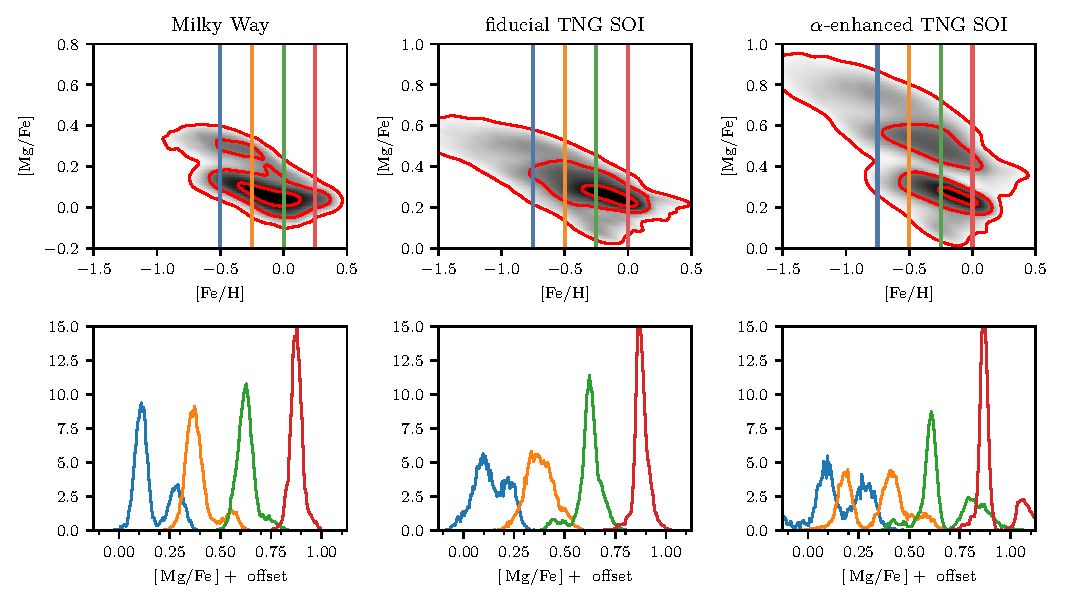
\includegraphics[width=\textwidth]{fig/392276.pdf}
  \caption{\textbf{Test.}}
  \label{fig:fig1}
\end{figure*}

\begin{figure*}
  \centering
  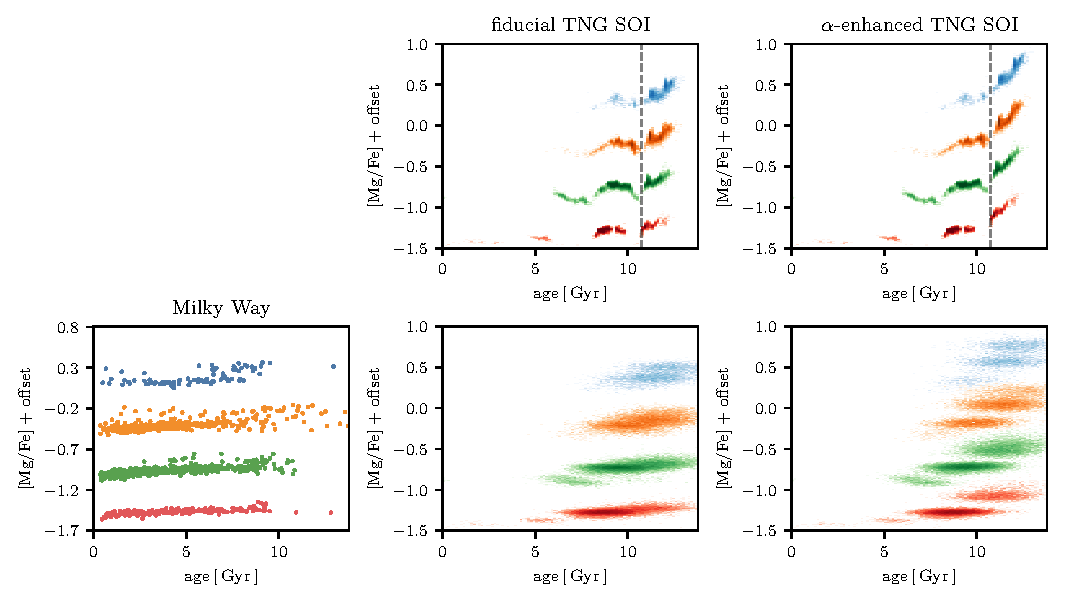
\includegraphics[width=\textwidth]{fig/392276_alpha.pdf}
  \caption{\textbf{Test.}}
  \label{fig:alpha}
\end{figure*}

\begin{figure}
  \centering
  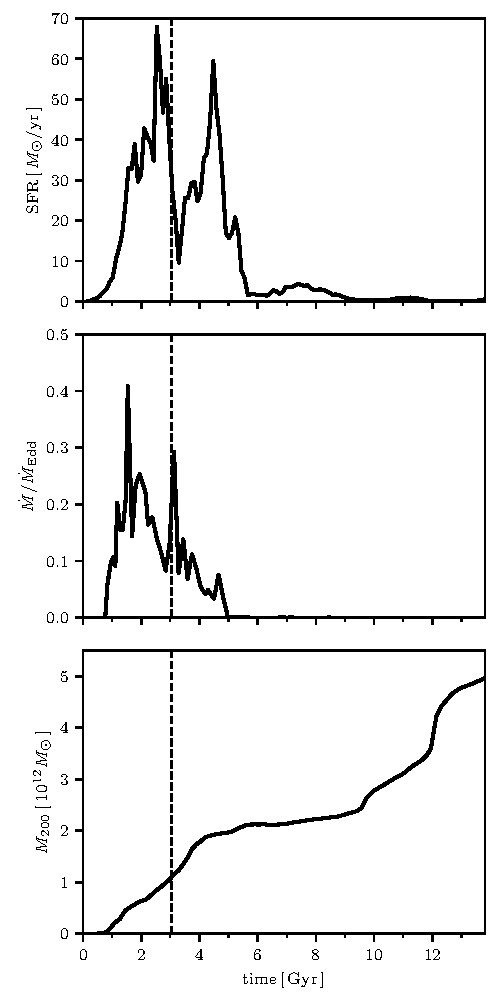
\includegraphics[width=\columnwidth]{fig/392276_SFH_AGN_M200.pdf}
  \caption{\textbf{Test.}}
  \label{fig:history}
\end{figure}

\begin{figure}
  \centering
  \includegraphics[width=\columnwidth]{fig/mgfe_vice.pdf}
  \caption{\textbf{Test.}}
  \label{fig:vice}
\end{figure}

The main result of our paper is given in Figure~\ref{fig:fig1}. Here, we compare the abundance plane in the Milky Way (left column) to that in our subhalo of interest (middle column). The colored vertical lines show 1D conditional histograms at $\FeH=-0.75$, $-0.5$, $-0.25$, and $0$ \red{check}. The Milky Way shows a clear bimodal population, with a high-$\alpha$ sequence most clearly distinct from the low-$\alpha$ sequence at low metallicity. The two sequences merge around solar metallicity.

Our subhalo of interest, on the other hand, does not show a clearly bimodal structure in the fiducial simulation (middle column). There is some structure in the $\FeH=-0.75$ and $\FeH=0$ bins, but the peaks are close together ($<0.1\dex$) and the trough-to-peak ratio is high ($\sim1/2$ and $1/5$, respectively). It is not obvious that this distribution would have any structure with observational errors.

The right panel of Figure~\ref{fig:fig1} shows the same distribution as in the middle panel, but with an artificial declination in \MgFe{}. Star particles are given an additive offset of $0.1\times\left(t_{1.5}-t_{\textrm{form}}\right)$, where $t_{1.5}$ is the age of the universe at $z=1.5$ and $t_{\textrm{form}}$ is the formation time of the star particle. Only stars formed before $z=1.5$ are shown. Here, one can see a striking multimodal structure with three clear modes at $\MgFe\sim0.8$, $0.5$, and $0.2\,\dex$. These modes display more contrasted structure, with the distance between modes increasing (to $\sim0.2\,\dex$) as well as the trough-to-peak ratio decreasing to $\sim0.4$ between the $0.8$ and $0.5$ modes and practically vanishing between the $0.5$ and $0.2$ modes.

\subsection{Time Dependence}\label{sec:timedep}

\section{Discussion}\label{sec:disc}
In Figure~\ref{fig:fig1}, we compared the abundance plane between the Milky Way and our subhalo of interest. The result is quite simple, and indicates a fairly straightforward conclusion: multimodality is enhanced when \alphaFe{} more strongly declines with time. 

\subsection{Cause of $\alpha$ Decline}\label{ssec:sfe}
As discussed in Section~\ref{sec:intro}, it has long been known that the \alphaFe{} ratio should decline with time \red{cite}. This declination is caused by the relative enrichment contribution between Type II and Type Ia SNe, with the former contributing the bulk of the $\alpha$-elements and both contributing to Fe. However, this picture is complicated by the details of galaxy evolution. Inflows and outflows, radial gas transfer, and unmixed local enrichment all have a strong effect on the \alphaFe{} ratio.

A detailed accounting of all these processes is beyond the scope of this work, and much of it is impossible with the sparse snapshot spacing in TNG. However, we do offer one possible explanation for the relatively minor declination of \alphaFe{} in the simulation: the SFE at high surface densities in TNG is too low.

First, we demonstrate the impact of the SFE on the \alphaFe{} ratio using a simple one-zone chemical evolution model with the publicly available code \texttt{VICE}. The details of our setup is given in Section~\red{X}. We vary the star formation timescale, $\tau_{*}=M_{\textrm{gas}}/\textrm{SFR}$, and examine the impact on the \MgFe{} ratio asa function of time. We find that shorter star formation timescales lead to a more rapid reduction in \MgFe{}. A close match to our subhalo of interest in TNG is not attempted.

In TNG, the SF timescale is set to a fixed value of $2.2\,\Gyr$. However, this value is the SF timescale used to set the SFR of an individual cell. What is relevant for comparison to these models is the SF timescale averaged over some well-mixed region. 

\subsection{Full Sample}\label{ssec:fullsamp}

A version of Figure~\ref{fig:fig1} for the rest of the subhalos in our original sample are given in the Appendix. They display a variety of morphologies, likely arising from a similar variety of processes. They are the subject of continuing work.



\begin{acknowledgements}
This work has made use of data from the European Space Agency (ESA) mission {\it Gaia} (\url{https://www.cosmos.esa.int/gaia}), processed by the {\it Gaia} Data Processing and Analysis Consortium (DPAC, \url{https://www.cosmos.esa.int/web/gaia/dpac/consortium}). Funding for the DPAC has been provided by national institutions, in particular the institutions participating in the {\it Gaia} Multilateral Agreement.
\end{acknowledgements}

\bibliography{ref}{}
\bibliographystyle{aasjournal}

% \input{src/app.tex}

\end{document}
